% TEMPLATE for Usenix papers, specifically to meet requirements of
%  USENIX '05
% originally a template for producing IEEE-format articles using LaTeX.
%   written by Matthew Ward, CS Department, Worcester Polytechnic Institute.
% adapted by David Beazley for his excellent SWIG paper in Proceedings,
%   Tcl 96
% turned into a smartass generic template by De Clarke, with thanks to
%   both the above pioneers
% use at your own risk.  Complaints to /dev/null.
% make it two column with no page numbering, default is 10 point

% Munged by Fred Douglis <douglis@research.att.com> 10/97 to separate
% the .sty file from the LaTeX source template, so that people can
% more easily include the .sty file into an existing document.  Also
% changed to more closely follow the style guidelines as represented
% by the Word sample file. 

% Note that since 2010, USENIX does not require endnotes. If you want
% foot of page notes, don't include the endnotes package in the 
% usepackage command, below.

% This version uses the latex2e styles, not the very ancient 2.09 stuff.
\documentclass[letterpaper,twocolumn,10pt]{article}
\usepackage{usenix,epsfig,endnotes,mathtools}
\begin{document}

%don't want date printed
\date{}

%make title bold and 14 pt font (Latex default is non-bold, 16 pt)
\title{\Large \bf EDEALS:  Electricity Demand-response Easy Adjusted Load Shifting  }

%for single author (just remove % characters)
%\author{
%{\rm Will McFadden}\\
%University of Chicago
%\and
%{\rm Ray Parpart}\\
%University of Chicago
%\and
%{\rm Anita Nikolich}\\
%Mogilner Institute
%} % end author

\maketitle

% Use the following at camera-ready time to suppress page numbers.
% Comment it out when you first submit the paper for review.
%\thispagestyle{empty}


\subsection*{Abstract}
Energy demand response presents a highly cost-effective means to improve the sustainability of data centers whenever there is flexibility in task scheduling.  This paper presents an empirical study in the area of data center demand response, with the goal of cost savings on electricity bills for small to medium size data centers drawing 1-5 MegaWatts. Using the Slurm resource manager, we demonstrate a methodology for energy aware scheduling by flexibly reducing compute cycles at times of peak energy demand.  Simply reducing the pool of available servers during peak energy demand results in tangible cost savings through reduced power consumption of the server cluster, with minimal performance degradation to users. We have developed a data processing pipeline to determine the potential cost savings of partial data center shutdown to enable demand-response load shifting. As our baseline, we measured the power draw and job scheduling delay of a small-scale test cluster undergoing a temporary power down. We then model a production cluster's performance in response to a realistic energy constraint imposed by a utility provider.  We quantify a typical annual cost savings on electricity of 7\% while only causing 16 hours of total increased wait time (0.1\%) throughout the entire year.


\section{Introduction}

Data centers in the US consume an estimated 91 billion kilowatt-hours yearly, equivalent to the annual output of 34 large coal-fired power plants.\cite{Delforge2014} These same estimates show that only 6-12\% of the electricity is used for powering servers while the rest is used to keep machines idling, wasting resources and money in the process. Data center electricity is not inexpensive, costing American businesses \$13 billion annually in electricity bills.\cite{Delforge2014} Because cost is a strong motivating factor for businesses and universities, we consider data center energy efficiency in the context of cost savings for data center operations. \\

\begin{figure}[t]
	\begin{center}
		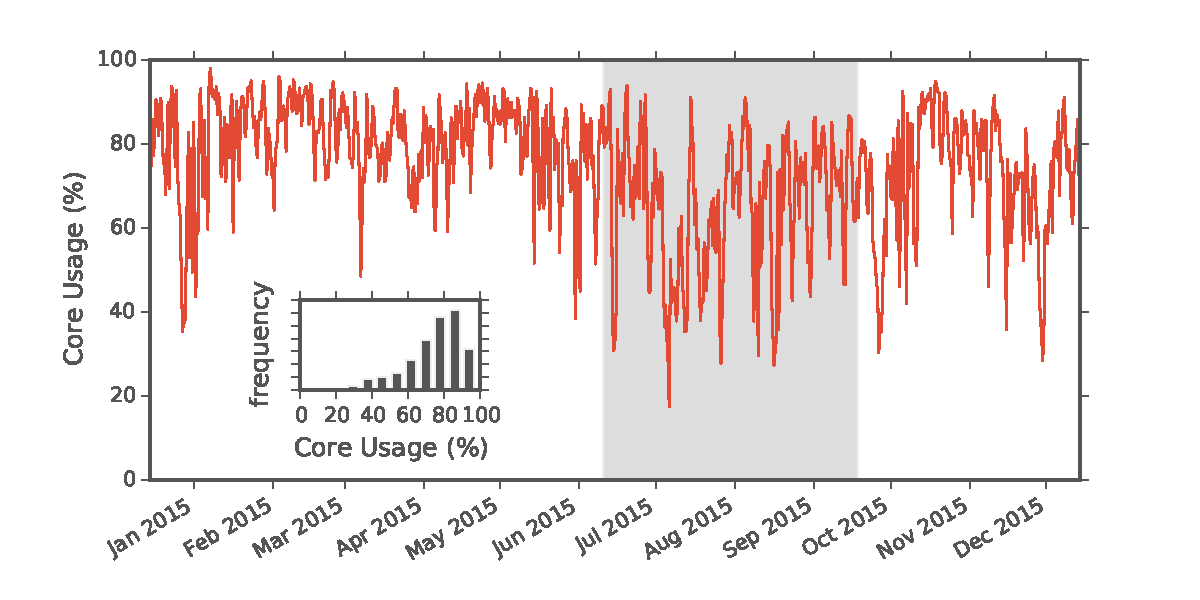
\includegraphics[scale=0.38]{pwr_model_ins}
		%		\begin{picture}(300,150)(0,200)
		%		\put(-15,-30){\special{psfile = fig1.ps hscale = 50 vscale = 50}}
		%		\end{picture}\\
	\end{center}
	\caption{Average core usage for a 244 node shared HPC partition in the Midway cluster. Insert shows usage statistics histogram.}
	\label{prw_model_ins}
\end{figure}

Demand response (DR) programs provide incentives to induce dynamic management of customers’ electricity load in response to power supply conditions, for example, reducing their power consumption in response to a request from the utility.\cite{7039172} Anita can you add something around here that points out how demand response also increases the “sustainability” of the datacenter beyond just cost reduction.Many energy providers have Voluntary Load Response (VLR) programs, which encourage commercial consumers to reduce power demands during peak periods, such as particularly hot summer days. Participants are given between one and four hours’ notice of a request to shed some of their electric load, with two and eight hours of participation and the expectation to shed at least 10 kilowatts. We are interested in exploring more active ways in which to participate in electricity demand response programs while impacting the users minimally.   \\

In many university data centers, a significant portion of the data center is dedicated to high performance research computing which is typically Tier 1. While these jobs take longer periods of time to complete, they are less time sensitive and more flexible than systems which support core business functions such as the university's email.  We wish to use the flexibility in scheduling of these jobs to reduce energy consumption of university data centers during periods of peak energy demand. \\  

As shown in the example core usage data of Figure \ref{prw_model_ins}, although the typical average usage during the school year is a fairly standard 80\%, the averaged workload can fall to 65\% of full capacity in the hottest summer months from June to September. These months also present the period of greatest electricity demand due largely to increased usage of air conditioning. This presents a valuable opportunity to potentially curtail electricity use in demand response scenarios by shifting load off of the peak periods of energy price.  Toward this aim, this paper is our attempt to estimate the economic savings, feasibility, and any potential user impact from full or partial cluster shutdown during periods of increased energy demand.


\subsection{Alternative Demand Response Options in Data Centers}

Although we focus on load shifting for our study, we wish to point out prior work on alternative strategies for demand response. \\

\textbf{Facility changes} A study by Lawrence Berkeley National Laboratory (LBNL) found that 5\% of the data center load can typically be shed in 5 minutes and 10\% of the load can be shed in 15 minutes without changes to how the IT workload is handled, i.e., via temperature adjustment and other building management approaches\cite{Ghatikar2012}. Most data centers have local power due to a backup generator, which could also be used to absorb some load during peak time \cite{Liu2013}. More recently, methods of energy storage have been proposed\cite{Narayanan2014} in which UPS batteries are re-purposed for provisioning during periods of peak demand in addition to their primary purpose of backup power. However, these methods all entail manual intervention, with close monitoring and control.

\textbf{Power capping} is a strategy by which to run data center equipment within a set of constraints which assume the electricity draw for the data center as a whole cannot grow any larger. Some examples of this include and turning off or constraining CPU/GPU power consumption to values below the CPU Thermal Design Power (TDP) value, which requires less voltage. Many equipment manufacturers - including IBM, Intel and AMD - have implemented power capping technology that can be monitored at the processor level and applied at the rack level. One approach to power capping is Dynamic Voltage/Frequency Scaling (DVFS). However, as noted by Roundtree\cite{Roundtree2012}, no machine in the Top 500 list of supercomputers makes use of DVFS to save power or energy since the performance impact and the amount of power and energy saved was highly application dependent. Power capping doesn’t necessarily equate to energy efficiency nor cost savings.

\textbf{Schedulers} Zhou et al\cite{Zhou2014} present a method for power-aware scheduling by using a combination of a scheduling window and 0-1 knapsack model, which shows promise. However, since SLURM is our scheduler, we decided to focus solely on SLURM. Bodas et al\cite{Bodas2014} demonstrate an integration of power capping into a power-aware scheduler, with the overall goal of maintaining average system power within a budget. Their work demonstrates that SLURM’s auto mode can be used to maximize available power.  

\begin{figure}[t]
	\begin{center}
		
				\begin{picture}(300,100)(20,200)
				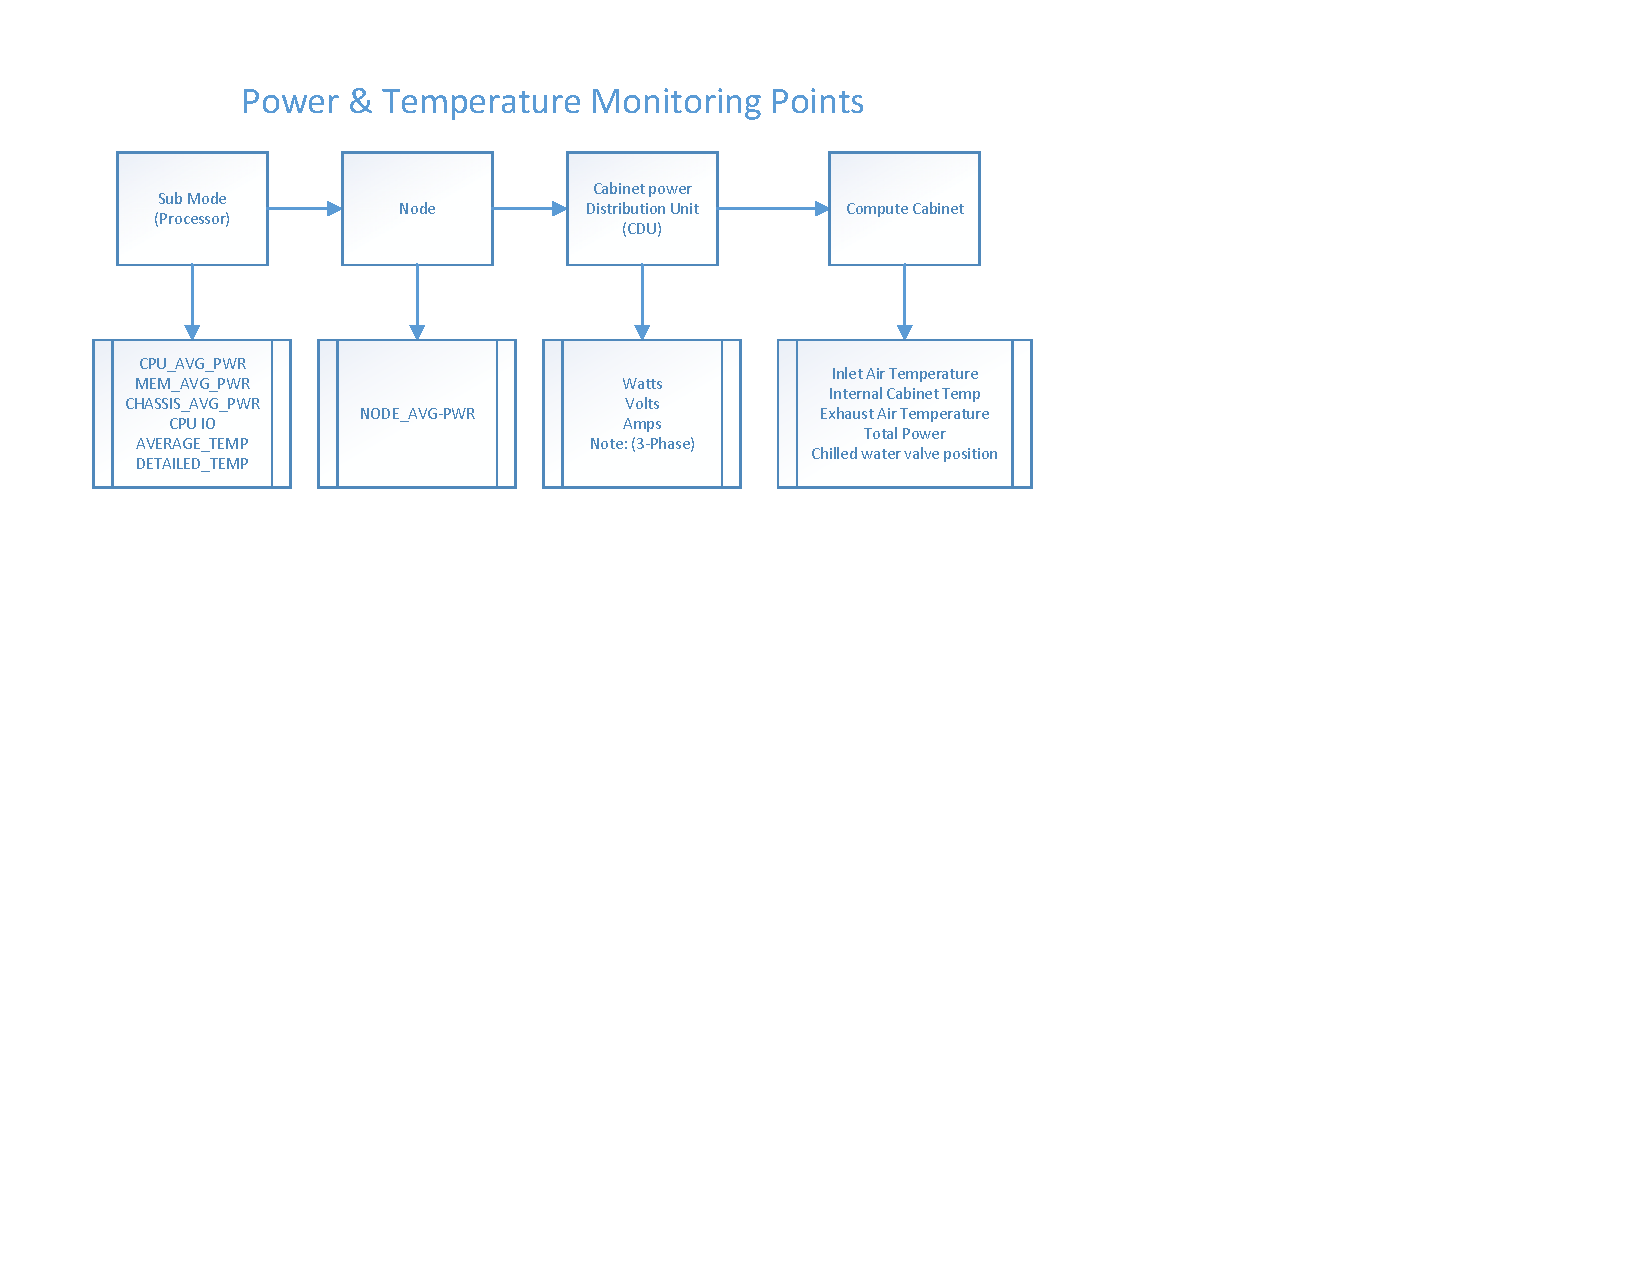
\includegraphics[scale=0.50]{ray_fig}
				\end{picture}\\
	\end{center}
	\caption{Energy monitoring framework.}
	\label{ray_fig}
\end{figure}


\section{Problem Statement}

Can load shifting of high performance computing tasks save universities money in energy demand response scenarios?  To explore the relative costs of implementing load shifting in demand response scenarios, we have expressed the problem by modeling total dollar cost.  We wish to use this framework to explore the optimization of price in the presence of various data center usage statistics and price fluctuation schemes.

\subsection{Modeling Energy Costs}

We generate a model total cost function composed of a fixed cost for purchasing and maintaining nodes plus a variable cost dependent on data center power usage and energy prices.  We wish to minimize the cost function

$$C = p_n T n_{max} + \int_0^T dt \cdot p(t)\left (n(t)u(t)+ u_w \frac{\Delta n(t) }{\Delta t} \right )  $$

where $p(t)$ is the price of power at time $t$, $0<n(t)<n_{max}$ is the number of running nodes, $u(t)$ is the average node power usage, $u_w$ is the wasted power from turning on a node, $p_n$ is the amortized lifetime cost of purchasing a node, and $n_{max}$ is the total number of nodes in the cluster.  

Based on our cluster usage statistics, we approximate that compute cycles are roughly interchangeable and that the main determiner of power usage is simply the CPU utilization of the node. In this case, node power usage takes the form

$$u(t) = u_0 + u_v \cdot r(t)$$

where $0<r(t)<1$ is the fraction of CPU usage, $u_0$ is the cost of an idling node and $u_v$ is the variable cost for doing $r$ work on a machine.

We wish to minimize the cost function $C$ subject to the constraint that the sum of the submitted CPU cycles, $S$, are all completed after a period T.

$$\int_0^T dt \cdot n(t)r(t) = S$$

\begin{figure}[t]
	\begin{center}
		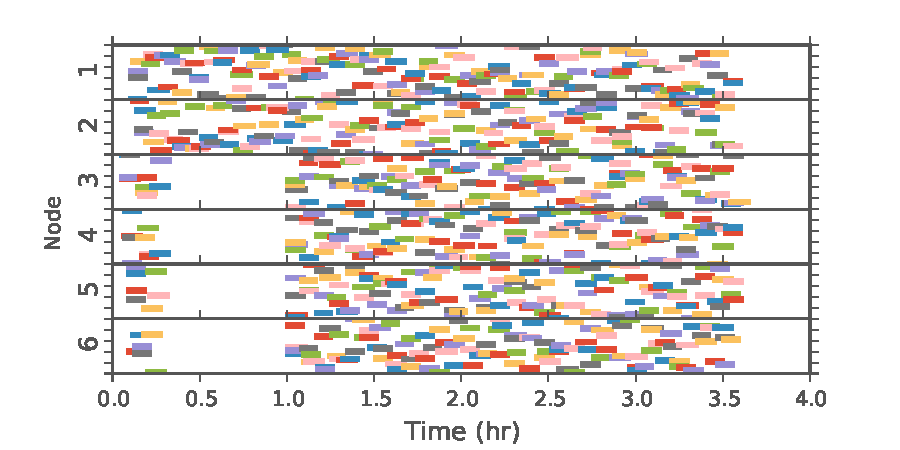
\includegraphics[scale=0.55]{usage_viz4}
		%		\begin{picture}(300,150)(0,200)
		%		\put(-15,-30){\special{psfile = fig1.ps hscale = 50 vscale = 50}}
		%		\end{picture}\\
	\end{center}
	\caption{Diagram of job scheduling during a four node temporary shutdown experiment. Each colored rectangle displays the execution time of a single LAMPPS test job running for approximately 5 minutes.}
	
\end{figure}

\begin{figure}[t]
	\begin{center}
		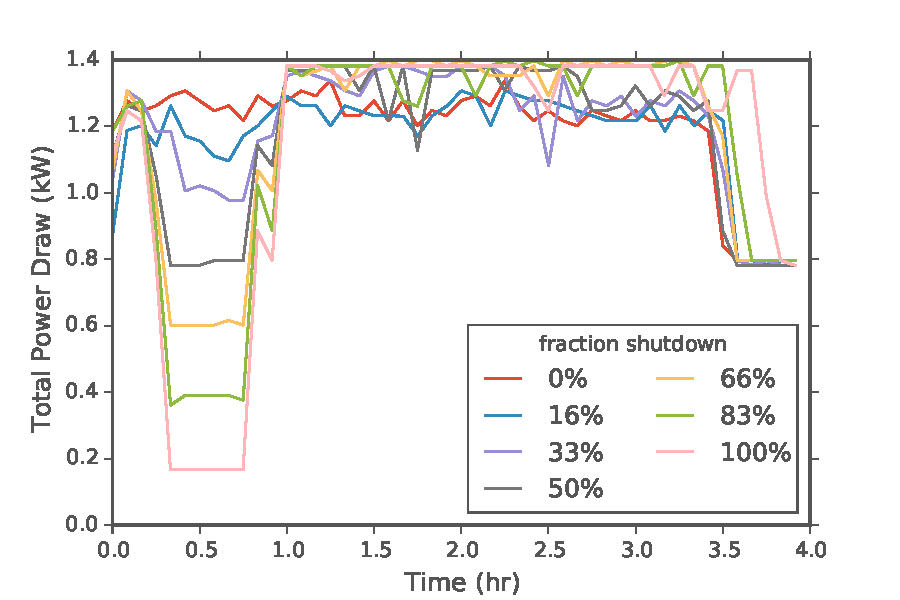
\includegraphics[scale=0.55]{power_viz}
		%		\begin{picture}(300,150)(0,200)
		%		\put(-15,-30){\special{psfile = fig1.ps hscale = 50 vscale = 50}}
		%		\end{picture}\\
	\end{center}
	\caption{Total power consumed during experiments where variable numbers of machines were shut down during simulated peak pricing.}
	\label{power_viz}
\end{figure}

\subsection{Response to a Temporary Price Spike}

In particular, we wish to use this framework to determine how to run our data center in the situation where every $T$ days, we see a "price spike" from $p_0$ to $p_s$, lasting time period $t_s$.  This condition is highly similar to the one facility managers face when utility provides impose usage tariffs during peak energy demand periods.

In this situation, the number of running machines will change stepwise between a high number of running machines, $n_H=n_{max}$, and a low number of running machines, $n_L$, and a high and low CPU utilization $r_H=1$, $r_L$, with a corresponding $u_H$ and $u_L$ as defined above.  The high usage will occur during the cheap energy supply, and the low usage will occur during the price spike.  Therefore we can rewrite our cost function as 

\begin{equation}
\begin{multlined}
	C = p_n n_H T + p_0 (u_0 + u_v) n_H (T-t_s) \\
	+ p_s (u_0 + u_v r_L) n_L t_s + p_0 u_w (n_H-n_L)
\end{multlined}
\end{equation}

with the constraint

\begin{equation}
n_H (T-t_s) + n_L r_L t_s = S
\end{equation}

Inserting the constraint into our cost function to replace $r_L$ yields 

\begin{equation}
\begin{multlined}
C = p_s u_v S + n_L \cdot( p_s u_0 t_s - p_0 u_w t_w) \\
+ n_H \cdot (p_n T + p_0 u_w t_w -(\Delta p u_v - p_0 u_0)(T-t_s))
\end{multlined}
\end{equation}
where we've introduce the price difference, $\Delta p = p_s - p_0$.

We can analyze the change in costs as a function of $n_L$ and $n_H$ to determine the optimal cluster setup for known variables, $t_s$, $p_s$, $p_n$, $p_0$, $u_0$, $u_v$, and $u_w$. 

From this analysis, whenever $ p_s u_0 t_s < p_0 u_w t_w$, the cost of powering off nodes exceeds the cost of running those nodes idle so $n_L = n_H$ and $r_L = S/n_H t_s - (T-t_s)/t_s$. Otherwise powering off nodes saves money so the nodes that remain on run at full capacity $r_L = 1$, and $n_L$ is minimized subject to constraints giving $n_L = S/t_s - n_H(T-t_s)/t_s$.

If we can freely choose $n_H$ to optimize cost, then whenever $(\Delta p u_v - p_0 u_0)(T-t_s) > p_n T + min(p_0 u_w t_w,p_s u_0 t_s)$, we would increase $n_H$ (i.e. buy more machines) until all the work is done during the cheap energy period. Therefore $n_H = S/(T-t_s)$ and either $n_L$ or $r_L$ is $0$.  Otherwise, the cost of new machines is more than any cost savings achieved from exploiting the price difference, and we would simply ignore the price spike (i.e. set $n_H = n_L = S/T$ and $r_L = 1$).

% you can also use the wonderful epsfig package...
\begin{figure}[t]
	\begin{center}
		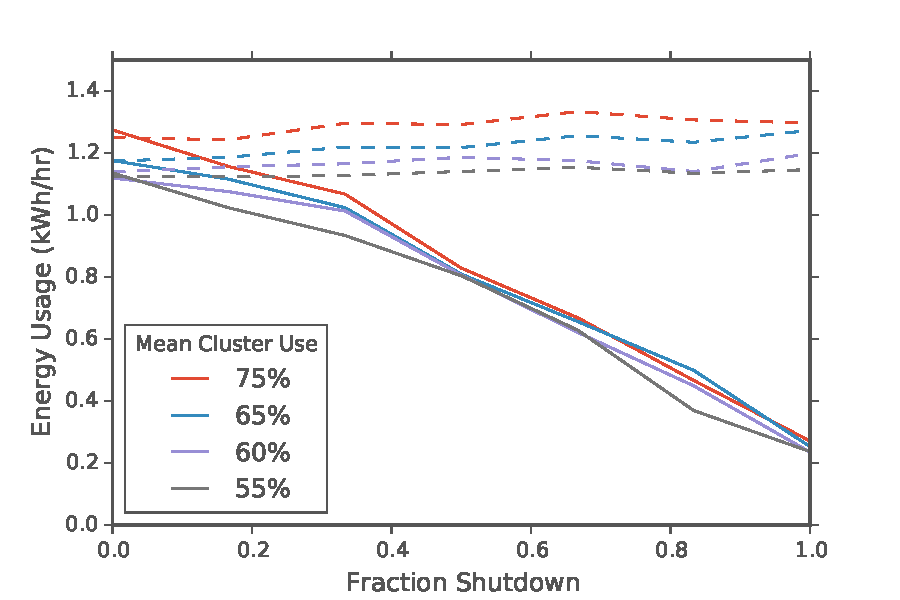
\includegraphics[scale=0.55]{down_v_pow}
		%		\begin{picture}(300,150)(0,200)
		%		\put(-15,-30){\special{psfile = fig1.ps hscale = 50 vscale = 50}}
		%		\end{picture}\\
	\end{center}
	\caption{Energy usage of test cluster during partial shutdown experiments.  Solid lines indicate power usage during the shutdown, while dashed lines indicate power usage after returning to full operation.}
	\label{down_v_pow}
\end{figure}

% you can also use the wonderful epsfig package...
\begin{figure}[t]
	\begin{center}
		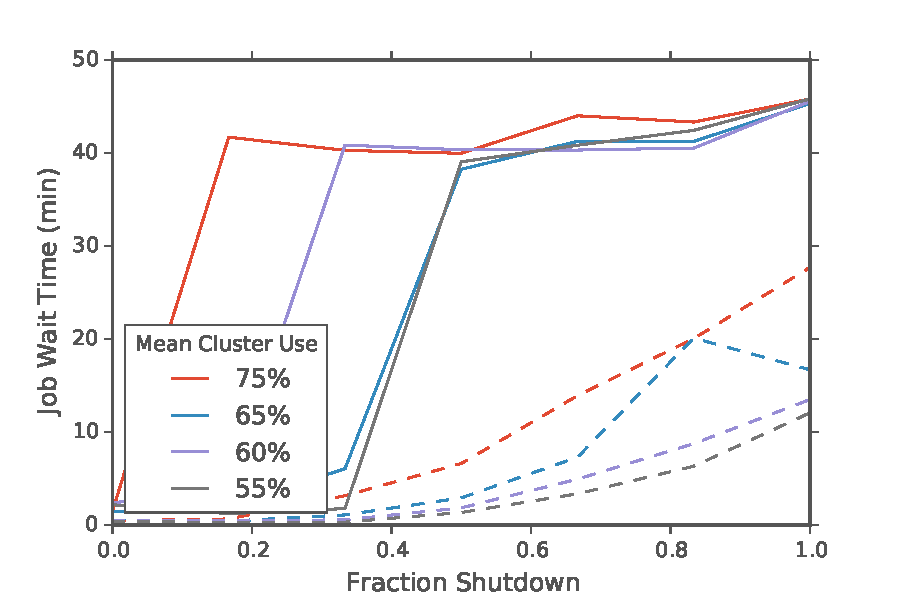
\includegraphics[scale=0.55]{down_v_wait}
		%		\begin{picture}(300,150)(0,200)
		%		\put(-15,-30){\special{psfile = fig1.ps hscale = 50 vscale = 50}}
		%		\end{picture}\\
	\end{center}
	\caption{Maximum (solid) and mean (dashed) job wait times during partial shutdown experiments.}
	\label{down_v_wait}
\end{figure}

\section{EDEALS: Electricity Demand-response Easy Adjusted Load Shifting}

For a data center manager to use the above model to determine their cost savings, they must collect and analyze usage and power data on their system.  We have built a cluster data processing pipeline, EDEALS, to assess the magnitude of potential savings available from a full or partial cluster shutdown.  We combine SLURM job scheduling, node level IMM power and usage metrics, and cabinet level CDU measurements to determine the optimum magnitude of demand response cluster shutdowns.  

Here we describe our data center instrumentation, so that we ensure accurate measurements of performance of the workload management system and HPC cluster alone without the influence of extraneous components. Since our focus is the HPC cluster and SLURM manager, we need to ensure those components alone affect the reduced data center utility bill.  As depicted in Figure \ref{ray_fig}, we take measurements at the core, node, rack, and cabinet level.  These data are combined to detect power losses at each step and to determine the correlation between the power measurements at the machine level and the true power draw at the facility level.

Combining this data with electricity pricing statistics from utility managers allows system administrators to determine when and by how much to reduce their power usage to save money.  We have built a set of scripts particular to our system to implement machine level power down in response to predicted energy peaks.  At the end of the peak energy period the machines automatically reboot and are added by to SLURM’s available server pool.  At this time, these power cycling scripts are manually executed by system administrators after evaluation of the likelihood of near-term energy demand peaks.  However, as more data centers begin to implement smart metering, it will become possible to automate load shifting in response to real-time energy pricing indicators.  We look forward to continuing this as future work.





\section{Small-Scale Evaluation of EDEALS}

To test our load shifting scheme, we launched a series of small-scale experiments on a 6 machine test cluster using SLURM batch management system to schedule jobs. We wished to compare the energy savings and job wait times during a full or partial cluster shutdown in response to an energy price spike.

\subsection{Experimental Setup}

We measured the total energy use over a 3.5 hour window of which the first 30 minutes comprised a partial cluster shutdown, followed by a 15 minute powerup routine. We explored the impact of shutting down between one and all six nodes during the 30 minute window. The shutdown was carried out by fully powering nodes off.  We compared this to the energy usage without the partial shutdown.

Identical sample jobs were submitted to the cluster via SLURM scheduler at a constant rate to set the average cluster usage to approximately 55\%, 60\%, 65\% and 75\% capacity.  We used custom state control commands to set the power states of individual machines in the test cluster.  The SLURM scheduler automatically shifted queued jobs to run on the available machines, as shown in the example job schedule displayed Figure \ref{usage_viz} from a four node shutdown experiment. We used our EDEALS data analysis pipeline to measure the changes in energy usage and job wait time in the queue.

\subsection{Evaluation of Model Parameters}

Importantly, EDEALS allowed us to determine appropriate power parameters, $u_0$, $u_v$, and $u_w$ for both our test rack as well as a larger partition of the University of Chicago's Midway production cluster.  Figure \ref{pwr_proc} shows the measured relationship between CPU utilization and energy usage as determined from the machine level IPMI metric data.


\begin{figure}[t]
	\begin{center}
		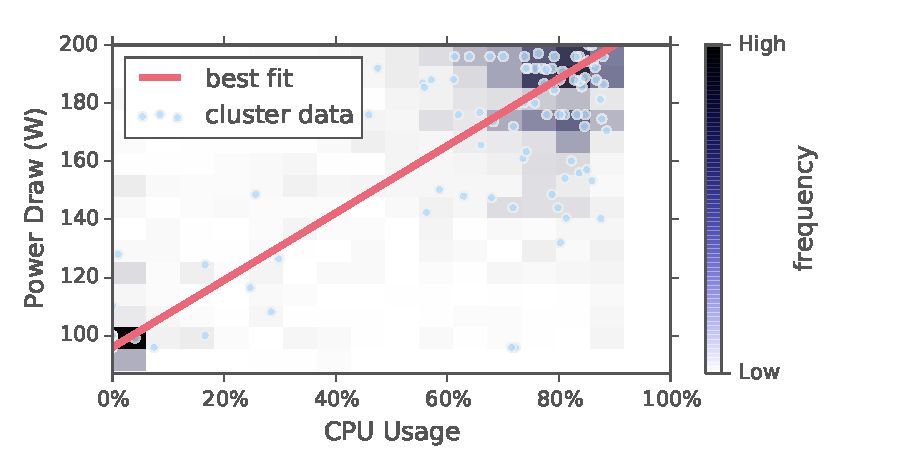
\includegraphics[scale=0.55]{pwr_proc}
		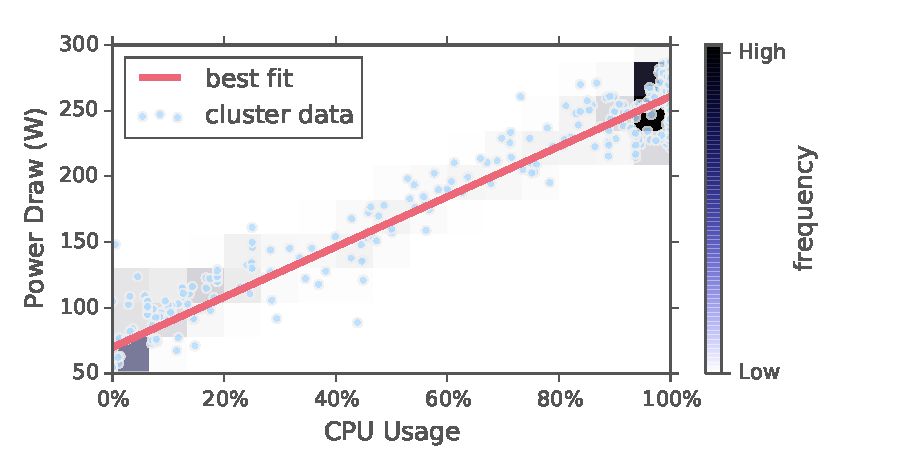
\includegraphics[scale=0.55]{pwr_proc_c}
		%		\begin{picture}(300,150)(0,200)
		%		\put(-15,-30){\special{psfile = fig1.ps hscale = 50 vscale = 50}}
		%		\end{picture}\\
	\end{center}
	\caption{Power data for test cluster (top) and production cluster (bottom) nodes in presence of variable usage. The slope and intercept of the line are used to determine $u_v$ and $u_0$ respectively. }
	\label{pwr_proc}
\end{figure}

\begin{figure}[t]
	\begin{center}
		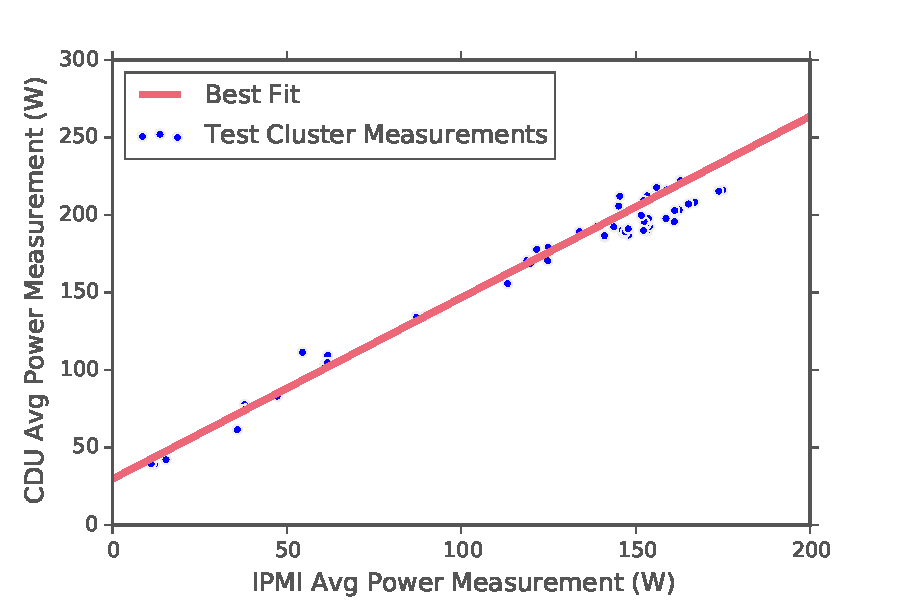
\includegraphics[scale=0.55]{ipmi_v_cdu}
		%		\begin{picture}(300,150)(0,200)
		%		\put(-15,-30){\special{psfile = fig1.ps hscale = 50 vscale = 50}}
		%		\end{picture}\\
	\end{center}
	\caption{Comparison between node level IPMI measurements and rack level CDU measurements. Best fit shows the model relationship used to convert IPMI data to estimated total power draw.}
	\label{ipmi_v_cdu}
\end{figure}

To account for losses not measured at the IPMI level, we compare the sum IPMI power usage to the rack level power monitoring.  This comparison revealed a correction factor of 1.25 between the IPMI measurement and the total rack level energy draw.  Using this corrected model, we were able to predict power consumption at the CDU level via CPU utilization under variable scheduler loads.

\subsection{Relative Energy Savings and Max Wait Times}

Our test cluster provided us with an important baseline in determining the effectiveness of a partial shutdown in reducing energy usage. As shown in Figure \ref{power_viz}, the total power draw from the test cluster was reduced dramatically during the shutdown period, and then returned to its baseline level.  

These experiments were repeated with different job submission rates such that the average CPU usage varied from 55\% to 75\%.  As shown in Figure \ref{down_v_pow}, the partial shutdowns reduced the total energy usage as measured at the CDU level.  Not surprisingly, the power usage during cluster shutdown for all usage levels converged to roughly the same value at the point where all remaining operational machines reached full capacity. Interestingly, the energy savings did not appear to be perfectly directly proportional to the fraction shut down.  In particular, there was residual energy use associated with our machine's low power state even when the cluster was entirely shut down.   

We also measured the difference between job submission and start time, as depicted in Figure \ref{down_v_wait}.  As one would expect, both mean and max wait times increased as the shutdown fraction grew and the effect was more pronounced when the cluster usage was higher.  However, we were pleasantly surprised to find that max wait times topped out at 45 minutes, which was the duration of the entire cluster down period.  This indicates that SLURM doesn't add too much additional overhead, and therefore, the worst-case user wait times would not exceed the total period that the cluster was shut down.

\section{Conclusion: Implication for An Operational HPC Datacenter}


In an HPC datacenter, the variable cost to supply electricity to a facility can be decomposed into both a nominal cost per kilowatt-hour and a procurement cost from the supplier.  Some suppliers impose a substantial procurement tariff based on electricity usage during the five, two hour long periods of highest demand in a year.  In this scenario, the savings of load shedding can be orders of magnitude higher than the nominal price per kilowatt-hour.  We estimate that by curtailing 1MW, 8 times per year, we can expect an annual savings of approximately \$100K, which in our case was roughly a 7% cost savings.  Approximating that the 8 curtailment days are roughly spread out over the 4 month period from June to September, we arrive at the system parameters listed in Table \ref{params}.



Combining these values with the power usage measurements from our production cluster, we can extrapolate the yearly savings based on fractional shutdowns of the data center.  In addition, using the wait time statistics from our test cluster we can also estimate the worst-case impact on user wait-times that these cluster shutdowns will incur.  We display this information in Figure \ref{final}, as a function of the fraction of the cluster that we would be theoretically willing to shut down.

\begin{figure}[t]
	\begin{center}
		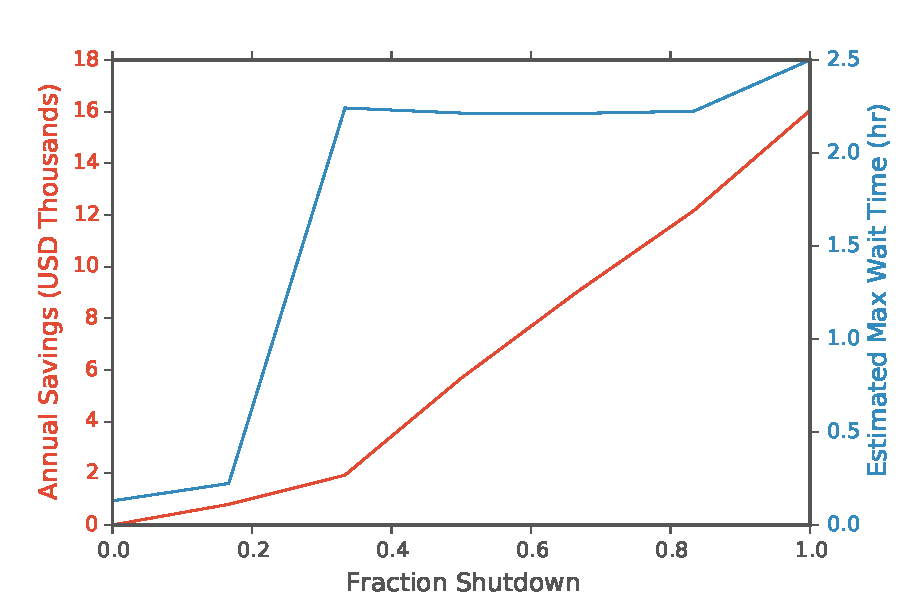
\includegraphics[scale=0.5]{final}
		%		\begin{picture}(300,150)(0,200)
		%		\put(-15,-30){\special{psfile = fig1.ps hscale = 50 vscale = 50}}
		%		\end{picture}\\
	\end{center}
	\caption{Estimated savings from partial cluster shutdowns. }
	\label{final}
\end{figure}


\begin{table}[]
	\centering
	\label{my-label}
	\begin{tabular}{|l|l|l|l|}
		\hline
		\textbf{$T$} & \textbf{$t_s$} & \textbf{$p_0$} & \textbf{$p_s$}  \\ \hline
		360 hr & 2 hr & \$0.03/kWh  & \$6.5/kWh    \\ \hline
	\end{tabular}
	\caption{Model parameters estimated for medium scale HPC datacenter.}
	\label{params}
\end{table}

\section{Acknowledgments}

Special thanks goes out to Brandon for all his work getting our test cluster set up as well as for his useful input on machine pricing information.  We also wish to thank Matt Beach for his invaluable knowledge on energy pricing mechanisms and university power plans.  Finally, we wish to thank Dr. Birali Runesha for his support in carrying out this project.

\section{Availability}

On our Github, we have provided all data collection scripts, analysis routines, and experimental setups, as well as detailed calculations and optimization methods for other price models.  

\begin{center}
{\tt https://github.com/rcc-uchicago/datacenter}
\end{center}

{\footnotesize \bibliographystyle{acm}
\bibliography{bibliography}}


\theendnotes

\end{document}







